\documentclass[border=6pt]{standalone}
\usepackage[T1]{fontenc}
\usepackage{amsmath, amssymb}
\usepackage{tikz}
\usetikzlibrary{shapes.multipart}

% --------------------------------------------------- Farben
\definecolor{physfill}{HTML}{DCE9F5}
\definecolor{physline}{HTML}{2C5F8A}

\newcommand{\cd}[1]{\texttt{#1}}

\begin{document}
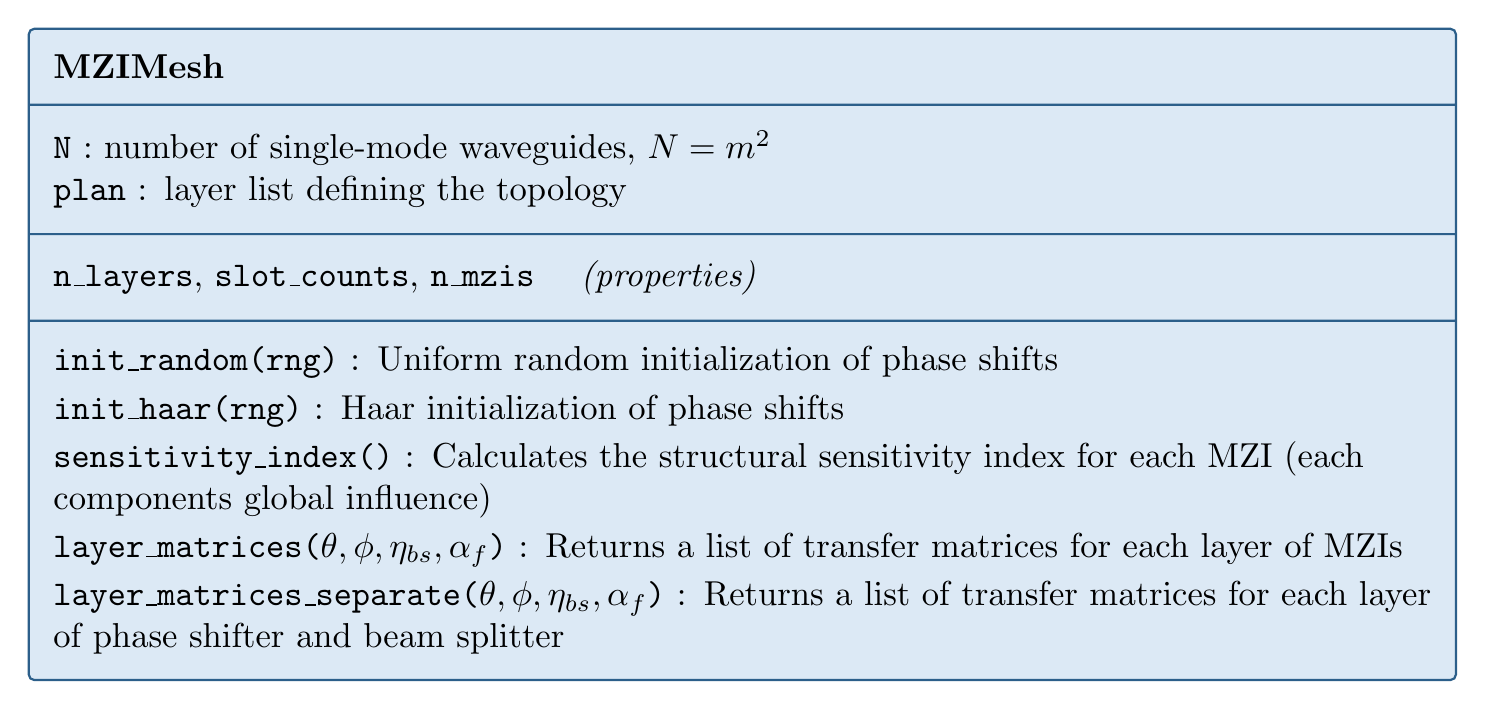
\begin{tikzpicture}[
    scale=1.25, transform shape,
    font=\normalsize,
    cls/.style   = {rectangle split, rectangle split parts=4,
                    rectangle split part align=left,
                    draw, thick, rounded corners=2pt,
                    fill=physfill, draw=physline,
                    text width=140mm, align=left, inner sep=2.5mm}
  ]

% =========================================================================
%  Das Klassendiagramm
% =========================================================================
\node[cls] (mesh)
  {\textbf{MZIMesh}\quad
   \nodepart{two}
   \cd{N} : number of single-mode waveguides, $N=m^{2}$\\
   \cd{plan} : layer list defining the topology\\[0.8mm]
   \nodepart{three}
   \cd{n\_layers}, \cd{slot\_counts}, \cd{n\_mzis}
     \quad\textnormal{\itshape (properties)}
   \nodepart{four}
   \cd{init\_random(rng)} : Uniform random initialization of phase shifts
   %$\rightarrow\ \theta\in[0,\pi],\ \phi\in[0,2\pi)$
   \\[0.7mm]
   \cd{init\_haar(rng)} : Haar initialization of phase shifts
   %$\rightarrow\ t=\xi^{1/\alpha}$
   \\[0.7mm]
   \cd{sensitivity\_index()} : Calculates the structural sensitivity index for each MZI (each components global influence)
   %$\rightarrow\
     %\alpha_{n\ell}=|I_{n\ell}|+|O_{n\ell}|-N-1$
     \\[0.7mm]
   \cd{layer\_matrices($\theta,\phi,\eta_{bs},\alpha_{f}$)} : Returns a list of transfer matrices for each layer of MZIs
     %$\rightarrow\ [\hat{M}_\ell]$
     \\[0.7mm]
   \cd{layer\_matrices\_separate($\theta,\phi,\eta_{bs},\alpha_{f}$)} : Returns a list of transfer matrices for each layer of phase shifter and beam splitter
    %$\rightarrow\ [\hat{M}_\theta,\hat{M}_\phi]$
    };

\end{tikzpicture}
\end{document}